\documentclass[12pt]{report}
\usepackage[utf8]{inputenc}
%\usepackage[14pt]{extsizes}
\usepackage{listings}
\usepackage{indentfirst}
\usepackage{geometry}
\usepackage{textcomp}
\usepackage{amssymb}
\usepackage{amsmath}
\usepackage{amsthm} 
\usepackage{caption}
\usepackage{misccorr}
\usepackage[noadjust]{cite}
\usepackage{cmap} 
\usepackage[T2A]{fontenc}
\usepackage[english, russian]{babel}
\usepackage{graphics}
\usepackage{graphicx}
\usepackage{textcomp}
\usepackage{verbatim}
\usepackage{makeidx}
\usepackage{float}
\usepackage{bm}
\usepackage{esint}
\usepackage{mathtools}
\usepackage{graphicx}
\usepackage{listings}
% Для листинга кода:
\lstset{ %
	language=python,                 % выбор языка для подсветки (здесь это С)
	basicstyle=\small\sffamily, % размер и начертание шрифта для подсветки кода
	numbers=left,               % где поставить нумерацию строк (слева\справа)
	numberstyle=\tiny,           % размер шрифта для номеров строк
	stepnumber=1,                   % размер шага между двумя номерами строк
	numbersep=5pt,                % как далеко отстоят номера строк от подсвечиваемого кода
	showspaces=false,            % показывать или нет пробелы специальными отступами
	showstringspaces=false,      % показывать или нет пробелы в строках
	showtabs=false,             % показывать или нет табуляцию в строках
	frame=single,              % рисовать рамку вокруг кода
	tabsize=2,                 % размер табуляции по умолчанию равен 2 пробелам
	captionpos=t,              % позиция заголовка вверху [t] или внизу [b] 
	breaklines=true,           % автоматически переносить строки (да\нет)
	breakatwhitespace=false, % переносить строки только если есть пробел
	escapeinside={\#*}{*)}   % если нужно добавить комментарии в коде
}


% plot
\usepackage{pgfplots}
\usepackage{filecontents}
\usetikzlibrary{datavisualization}

\usepackage[utf8]{inputenc}
%\usepackage[14pt]{extsizes}
\usepackage{listings}
\usepackage{indentfirst}
\usepackage{geometry}
\usepackage{textcomp}
\usepackage{amssymb}
\usepackage{amsmath}
\usepackage{amsthm} 
\usepackage{caption}
\usepackage{misccorr}
\usepackage[noadjust]{cite}
\usepackage{cmap} 
\usepackage[T2A]{fontenc}
\usepackage[english, russian]{babel}
\usepackage{graphics}
\usepackage{graphicx}
\usepackage{textcomp}
\usepackage{verbatim}
\usepackage{makeidx}
\usepackage{float}
\usepackage{bm}
\usepackage{esint}
\usepackage{mathtools}
\usepackage{graphicx}
\usepackage{listings}
% Для листинга кода:
\lstset{ %
	language=python,                 % выбор языка для подсветки (здесь это С)
	basicstyle=\small\sffamily, % размер и начертание шрифта для подсветки кода
	numbers=left,               % где поставить нумерацию строк (слева\справа)
	numberstyle=\tiny,           % размер шрифта для номеров строк
	stepnumber=1,                   % размер шага между двумя номерами строк
	numbersep=5pt,                % как далеко отстоят номера строк от подсвечиваемого кода
	showspaces=false,            % показывать или нет пробелы специальными отступами
	showstringspaces=false,      % показывать или нет пробелы в строках
	showtabs=false,             % показывать или нет табуляцию в строках
	frame=single,              % рисовать рамку вокруг кода
	tabsize=2,                 % размер табуляции по умолчанию равен 2 пробелам
	captionpos=t,              % позиция заголовка вверху [t] или внизу [b] 
	breaklines=true,           % автоматически переносить строки (да\нет)
	breakatwhitespace=false, % переносить строки только если есть пробел
	escapeinside={\#*}{*)}   % если нужно добавить комментарии в коде
}


% plot
\usepackage{pgfplots}
\usepackage{filecontents}
\usetikzlibrary{datavisualization}
\usetikzlibrary{datavisualization.formats.functions}
% Для измененных титулов глав:
\usepackage{titlesec, blindtext, color} % подключаем нужные пакеты
\definecolor{gray75}{gray}{0.75} % определяем цвет
\newcommand{\hsp}{\hspace{20pt}} % длина линии в 20pt
% titleformat определяет стиль
\titleformat{\chapter}[hang]{\Huge\bfseries}{\thechapter{.}}{10pt}{\Huge\bfseries}

\makeatletter
\def\@biblabel#1{#1. }
\makeatother

\usepackage{hyperref}

\newcommand{\specchapter}[1]{\chapter*{#1}\addcontentsline{toc}{chapter}{#1}}
\newcommand{\specsection}[1]{\section*{#1}\addcontentsline{toc}{section}{#1}}
\newcommand{\specsubsection}[1]{\subsection*{#1}\addcontentsline{toc}{subsection}{#1}}

% геометрия
\geometry{pdftex, left = 2cm, right = 2cm, top = 2.5cm, bottom = 2.5cm}

\titlespacing{\chapter}{0pt}{-30pt}{20pt}

\setcounter{tocdepth}{4} % фикс переноса 
\righthyphenmin = 2
\tolerance = 2048

\begin{document}
%\def\chaptername{} % убирает "Глава"
\thispagestyle{empty}
\renewcommand\bibname{Список литературы}

\vspace{\baselineskip}
\noindent \begin{minipage}{0.15\textwidth}
	
\includegraphics[width=\linewidth]{b_logo.jpg}
\end{minipage}
\noindent\begin{minipage}{0.9\textwidth}
	\centering
	\textbf{Министерство науки и высшего образования Российской Федерации}\\
	\textbf{Федеральное государственное бюджетное образовательное учреждение высшего образования}\\
	\textbf{«Московский государственный технический университет имени Н.Э.~Баумана}\\
	\textbf{(национальный исследовательский университет)»}\\
	\textbf{(МГТУ им. Н.Э.~Баумана)}
\end{minipage}

\noindent\rule{18cm}{3pt}
\newline\newline
\noindent ФАКУЛЬТЕТ $\underline{\text{«Информатика и системы управления»}}$ \newline\newline
\noindent КАФЕДРА $\underline{\text{«Программное обеспечение ЭВМ и информационные технологии»}}$\newline\newline\newline\newline\newline\newline\newline


\begin{center}
\Large\textbf{Лабораторная работа № 7}
\end{center}
\vspace{\baselineskip}
\noindent\textbf{Дисциплина} $\underline{\text{Анализ алгоритмов~~~~~~~~~~~~~~~~~~~~~~~~~~~~~~~}}$\newline\newline
\noindent\textbf{Тема} $\underline{\text{Поиск в словаре~~~~~~~~~~~~~~~~~~~~~~~~~~~~~~~~~~~~~~~~~~~~~~~}}$\newline\newline
\noindent\textbf{Студент} $\underline{\text{Воякин А. Я.~~~~~~~~~~~~~~~~~~~~~~~~~~~~~~~~~~~~~~~~~~~~~}}$\newline\newline
\noindent\textbf{Группа} $\underline{\text{ИУ7-54Б~~~~~~~~~~~~~~~~~~~~~~~~~~~~~~~~~~~~~~~~~~~~~~~~~~~~~~}}$\newline\newline
\noindent\textbf{Преподаватель} $\underline{\text{Волкова Л. Л. Строганов Ю.В.~~~~~~~~~~~~~~~~~~~~~~~~~~~~~~~~~~}}$\newline

\begin{center}
	\vfill
	Москва~---~\the\year
	~г.
\end{center}
\clearpage

\tableofcontents

\newpage
\chapter*{Введение}
\addcontentsline{toc}{chapter}{Введение}
Структура данных, позволяющая идентифицировать ее элементы не
по числовому индексу, а по произвольному, называется словарем или ассоциативным массивом. Каждый элемент словаря состоит из двух объектов:
ключа и значения. 

Ассоциативный массив с точки зрения интерфейса удобно рассматривать как обычный массив, в котором в качестве индексов можно использовать не только целые числа, но и значения других типов – например, строки \cite{dict}.
В данной лабораторной работе будут рассмотренны и реализованы такие алгоритмы поиска в словаре как:
\begin{enumerate}
	\item полный перебор;
	\item бинарный поиск;
	\item поиск по сегментам.
\end{enumerate}
\vspace{\baselineskip}

\textbf{Цель работы:} изучить и применить на практике алгоритмы поиска по словарю.\vspace{\baselineskip} 

\textbf{Задачи работы:}
\begin{enumerate}	
	\item Описать и реализовать алгоритмы полного перебора, двоичного поиска, поиска по сегментам.
	
	\item Провести сравнительный анализ алгоритмов поиска по словарю.
	
	\item Сделать выводы о применимости алгоритмов к решению задачи поиска по словарю.
\end{enumerate}


\chapter{Аналитическая часть}
В данном разделе содержится описание алгоритмов поиска по словарю.

\section{Алгоритм полного перебора}
Алгоритмом полного перебора называют метод решения задачи, при
котором по очереди рассматриваются все возможные варианты исходного
набора данных \cite{brute}. В случае словарей будет произведен последовательный перебор элементов словаря до тех пор, пока не будет найден необходимый.
Сложность такого алгоритма зависит от количества всех возможных решений, а время решения может стремиться к экспоненциальному времени
работы.

Пусть алгоритм нашёл элемент на первом сравнении (лучший случай), тогда будет затрачено $k_0 + k_1$ операций, на втором - $k_0 + 2 \cdot k_1$, на последнем (худший случай) - $k_0 + N \cdot k_1$. Если ключа нет в массиве ключей, то мы сможем понять это, только перебрав все ключи, таким образом трудоёмкость такого случая равно трудоёмкости случая с ключом на последней позиции. Средняя трудоёмкость может быть рассчитана как математическое ожидание по формуле (\ref{for:brute}), где $\Omega$ -- множество всех возможных случаев.

\begin{equation}
	\label{for:brute}
	\begin{aligned}
		\sum\limits_{i \in \Omega} p_i \cdot f_i = & (k_0 + k_1) \cdot \frac{1}{N + 1} + (k_0 + 2 \cdot k_1) \cdot \frac{1}{N+1} +\\
		& + (k_0 + 3 \cdot k_1) \cdot \frac{1}{N + 1} + (k_0 + Nk_1)\frac{1}{N + 1} + (k_0 + N \cdot k_1) \cdot \frac{1}{N + 1} =\\
		& = k_0\frac{N+1}{N+1}+k_1+\frac{1 + 2 + \cdots + N + N}{N + 1} = \\
		& = k_0 + k_1 \cdot \left(\frac{N}{N + 1} + \frac{N}{2}\right) = k_0 + k_1 \cdot \left(1 + \frac{N}{2} - \frac{1}{N + 1}\right)
	\end{aligned}
\end{equation}

\section{Алгоритм двоичного поиска}

Алгоритм двоичного поиска применяется к заранее упорядоченному словарю. 

При бинарном поиске искомый ключ сравнивается с ключом среднего элемента в словаре. Если они равны, то поиск успешен. В противном случае поиск осуществляется аналогично в левой или правой частях словаря \cite{binary}.

На каждом шаге осуществляется поиск середины отрезка по формуле (\ref{for:binary}).

\begin{equation}
	\label{for:binary}
	\begin{aligned}
		mid = \frac{left + right}{2}
	\end{aligned}
\end{equation}

Если искомый элемент равен элементу с индексом mid, поиск завершается.
В случае если искомый элемент меньше элемента с индексом mid, на место mid перемещается правая граница рассматриваемого отрезка, в противном случае — левая граница.

Поиск в словаре с использованием данного алгоритма в худшем случае (необходимо спуститься по двоичному дереву от корня до листа) будет иметь трудоемкость $O(log_2 N)$, что быстрее поиска при помощи
алгоритма полного перебора. Но стоит учитывать тот факт, что данный
алгоритм работает только для заранее упорядоченного словаря. В случае
большого объема данных и обратного порядка сортировки может произойти так, что алгоритм полного перебора будет эффективнее по времени, чем
алгоритм двоичного поиска.


\section{Алгоритм частотного анализа}

Алгоритм на вход получает словарь и на его основе составляется частотный анализ. По полученным значениям словарь разбивается на сегменты так, что все элементы с некоторым общим признаком попадают в один сегмент (для строк это может быть первая буква, для чисел - остаток от деления) \cite{combi}. 

Сегменты упорядочиваются по значению частотной характеристики так, чтобы к элементам с наибольшей частотной характеристикой был самый быстрый доступ. Такой характеристикой может послужить, например, размер сегмента. Вероятность обращения к определенному сегменту равна сумме вероятностей обращений к его ключам, то есть $P_i = \sum_{j}p_j = N \cdot p$, где $P_i$ - вероятность обращения к $i$-ому сегменту, $p_j$ - вероятность обращения к $j$-ому элементу, который принадлежит $i$-ому сегменту. Если обращения ко всем ключам равновероятны, то можно заменить сумму на произведение, где $N$ - количество элементов в $i$-ом сегменте, а $p$ - вероятность обращения к произвольному ключу.

Далее ключи в каждом сегменте упорядочиваются по значению. Это необходимо для реализации бинарного поиска, который обеспечит эффективный поиск со сложностью $O(\log_2n)$, где $n$ - количество ключей в сегменте внутри сегмента.

Таким образом, сначала выбирается нужный сегмент, а затем в нем проводится бинарный поиск нужного элемента. Средняя трудоёмкость при множестве всех возможных случаев $\Omega$ может быть рассчитана по формуле (\ref{for:frequency}). 

\begin{equation}
	\label{for:frequency}
	\sum_{i \in \Omega}{\left(f_{\text{выбор сегмента i-ого элемента}} + f_{\text{бинарный поиск i-ого элемента}}\right)} \cdot p_i
\end{equation}


\section{Вывод}
В данном разделе были рассмотрены алгоритмы поиска по словарю.


\chapter{Конструкторская часть}
\addcontentsline{toc}{section}{Конструкторская часть}
В данном разделе содержатся схемы алгоритмов решения поиска по словарю и представлена структура рассматриваемого словаря.

\section{Структура словаря}

Словарь состоит из пар вида \texttt{<number - type>}, где \texttt{number} - номер счета, \texttt{type} - тип оплаты.

\section{Cхемы алгоритмов}

На рисунке \ref{fig:Brute} представлена схема алгоритма полного перебора.

\begin{figure}[H]
	\center{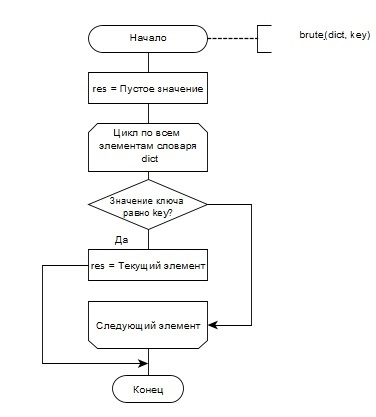
\includegraphics[scale=0.8]{schemaBrute.jpg}}
	\caption{Cхема алгоритма полного перебора.}
	\label{fig:Brute}
\end{figure}

\newpage
На рисунке \ref{fig:Binary} представлена схема алгоритма двоичного поиска.

\begin{figure}[H]
	\center{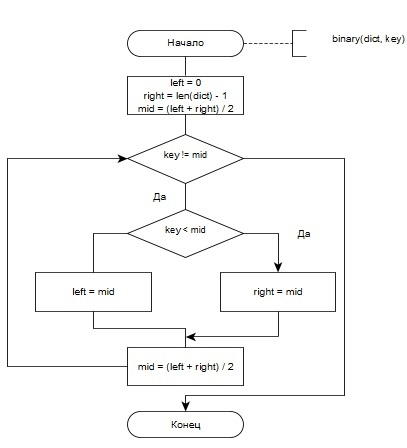
\includegraphics[scale=0.8]{schemaBinary.jpg}}
	\caption{Cхема алгоритма двоичного поиска.}
	\label{fig:Binary}
\end{figure}

\newpage
На рисунке \ref{fig:Combi} представлена схема алгоритма с использованием частотного анализа.

\begin{figure}[H]
	\center{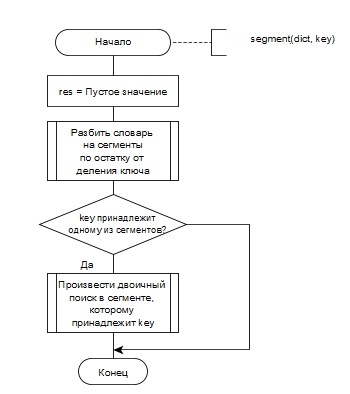
\includegraphics[scale=0.8]{schemaCombi.jpg}}
	\caption{Схема алгоритма с использованием частотного анализа.}
	\label{fig:Combi}
\end{figure}

\section{Вывод}
В данном разделе были представлены схемы алгоритмов поиска по словарю.


\chapter{Технологическая часть}
В данном разделе будут рассмотрены требования к программному обеспечению, средства реализации, представлен листинг кода, функциональное тестирование.

\section{Требования к программному обеспечению}
Требования к программе:

\begin{itemize}
	\item на вход подаётся словарь и значение ключа;
	\item на выходе — элемент словаря, значение ключа которого равно введенному. 
\end{itemize}

\section{Средства реализации}
В качестве языка программирования был выбран Python т.к. я хорошо знаю этот язык, он простой и лаконичный, имеющий немногословный и понятный синтаксис, похожий на псевдокод, обладающий сильной динамической типизацией, которая способствует быстрому написанию кода. 
 
Время  работы алгоритмов было замерено с помощью функции process\_time() из библиотеки time \cite{time}.

Для тестирования использовался компьютер на базе процессора Intel(R) Core(TM) i5-4200U, 2 ядра, 4 логических процессоров. 


\newpage
\section{Листинг кода}

В листинге \ref{lst:Brute} представлена реализация поиска по словарю с помощью алгоритма полного перебора.

\begin{lstlisting}[label={lst:Brute},caption=Реализация поиска по словарю с помощью алгоритма полного перебора.]
def brute(dictionary, number):
    for record in dictionary:
        if record['number'] == number:
            return record
    return None
\end{lstlisting} 

\vspace{\baselineskip}
В листинге \ref{lst:Binary} представлена реализация алгоритма двоичного поиска.
\begin{lstlisting}[label={lst:Binary},caption=Реализация алгоритма двоичного поиска.]
def binary(dictionary, number):
    left = 0
    right = len(dictionary) - 1

    if dictionary[left]['number'] > number or dictionary[right]['number'] < number:
        return None

    if dictionary[left]['number'] == number:
        return dictionary[left]
    if dictionary[right]['number'] == number:
        return dictionary[right]

    mid = (left + right) // 2
    res = dictionary[mid]['number']
    while number != res:
        if number < res:
            right = mid
        elif number > res:
            left = mid
        mid = (left + right) // 2
        res = dictionary[mid]['number']
    return dictionary[mid]
\end{lstlisting}

\newpage
В листинге \ref{lst:Analysis} представлена реализация алгоритма поиска по словарю с использованием частотного анализа. Словарь разбивается на сегменты так, что все элементы с одинаковым остатком от деления ключа попадают в один сегмент.
\begin{lstlisting}[label={lst:Analysis},caption=Реализация алгоритма поиска по словарю с использованием частотного анализа.]
def divide_dict(dictionary, segment_count):
    segment_list = [[] for _ in range(segment_count)]
    for record in dictionary:
        segment_list[record['number'] % segment_count].append(record)
    return segment_list


def segment(segment_list, number):
    if len(segment_list) == 0:
        return None
    return binary(segment_list[number % len(segment_list)], number)
\end{lstlisting}

\section{Функциональное тестирование}

Реализовано функциональное тестирование. Полученные результаты функций сравниваются с контрольными значениями. \vspace{\baselineskip}

Тестирование проходит по следующим данным:
\begin{itemize}
	\item ключ отсутсвует в словаре.
	\item ключ является первым элементом словаря.
	\item ключ является последним элементом словаря.
	\item ключ является произвольным элементом словаря.
\end{itemize}

В таблице \ref{tab1} представлено тестирование программы.

\newpage
\begin{table}
	\caption{Функциональное тестирование}
	\label{tab1}
	\begin{center}
		\begin{tabular}{ | c | c | c | c | c|}
			\hline
			\textbf{Ключ} & \textbf{Ожидаемый результат} & \textbf{Полный перебор} & \textbf{Бинарный поиск} & \textbf{Частотный анализ} \\ \hline
			'0' & 
			None &
			None &
			None &
			None  \\ \hline
			
			'1' & 
			{'Личные средства(банковский счет)'} &
			{'Личные средства(банковский счет)'} &
			{'Личные средства(банковский счет)'} &
			{'Личные средства(банковский счет)'}  \\ \hline	
			
			'1000' &
			{'За счет организации'} &
			{'За счет организации'} &
			{'За счет организации'} &
			{'За счет организации'}  \\ \hline	
			
			'992' &
			{'Материнский капитал'} &
			{'Материнский капитал'} &
			{'Материнский капитал'} &
			{'Материнский капитал'}  \\ \hline	
			
		\end{tabular}
		\end{center}
		
		\hfill
		
\end{table}	

Программа успешно прошла все тестовые случаи.

\section{Вывод}
В этом разделе обоснован выбор языка програмирования, описаны технические характеристики,приведены листинги кода реализованных алгоритмов. Программа прошла тестирование и работает правильно.

\chapter{Исследовательская часть}

В данном разделе приведены примеры работы программы, а также проведен сравнительный анализ алгоритмов по времени.
\section{Примеры работы}
На рисунках 4.1 - 4.2 приведены примеры работы программы. 

\begin{figure}[ht!]
	\center{
\includegraphics[scale=0.9]{pr1.png}}
	\caption{Пример работы программы (введённый ключ существует)}
\end{figure}

\begin{figure}[ht!]
	\center{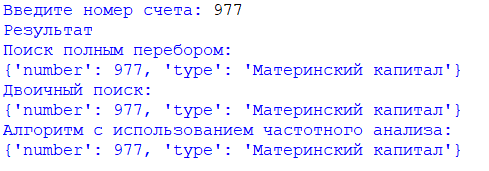
\includegraphics[scale=0.9]{pr2.png}}
	\caption{Пример работы программы (введённый ключ не существует)}
\end{figure}


\newpage
\section{Сравнение времени работы алгоритмов}
Для произведения замеров времени выполнения реализации алгоритмов будет использована формула: \begin{equation}\label{eq:fourierrow}
	t = \frac{T}{N}
\end{equation}
где t — среднее время выполнения алгоритма, N — количество замеров, T — время выполнения N замеров.  
Неоднократное измерение времени необходимо для получения более точного результа.  
Количество замеров взято равным 100. Для сравнения времени работы алгоритмов использовался словарь, состоящий из 1751 элемента. На рисунке 4.3 представлены графики времени работы алгоритмов поиска по словарю. Индекс ключа указан на горизонтальной оси.


\begin{figure}[ht!]
	\center{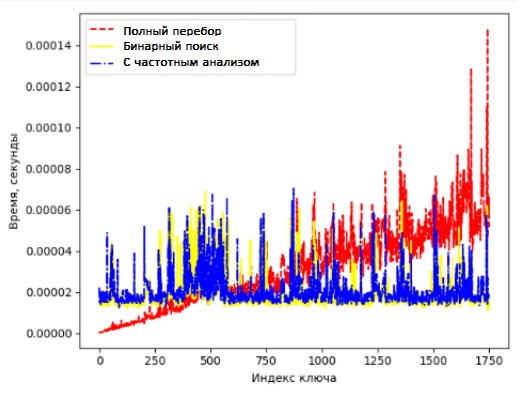
\includegraphics[scale=0.6]{time.jpg}}
	\caption{График зависимости времени работы алгоритмов от размера матрицы}
\end{figure}

Как можно наблюдать на графике, самый медленный алгоритм - алгоритм полного перебора. Время на в нём растет линейно и увеличивается с увеличением индекса элемента словаря. Алгоритм бинарного
поиска и алгоритм с использованием частотного анализа трятят примерно одинаковое количество времени, однако стоит учитывать, что они требуют дополнительных расходов времени на подготовку данных к работе с алгоритмом.
Однако в лучшем случае алгоритм полного перебора работает в 4 раза быстрее алгоритма двоичного поиска и алгоритма с использованием частотного анализа.

\newpage
\section{Вывод}
В данном разделе были приведены примеры работы программы, а также проведен сравнительный анализ алгоритмов по времени.

\newpage
\chapter*{Заключение}
\addcontentsline{toc}{chapter}{Заключение}
Цель работы достигнута. Получены практические навыки реализации алгоритмов поиска, а также проведен анализ времени их работы. Алгоритм полного перебора работает быстро в лучшем случае (когда искомые ключи находятся в самом начале словаря). Однако для работы лучше использовать алгоритм бинарного поиска или алгоритм с использованием частотного анализа. Сравнительный анализ по времени показал, что время их работы примерно одинаково, но алгоритм с использованием частотного анализа выигрывает в случае, если искомые ключи находятся в конце словаря.


\begin{thebibliography}{2}
	\addcontentsline{toc}{chapter}{Список литературы}
	
	\bibitem{dict} Словари (ассоциативные массивы) в Python [Электронный ресурс]. - Режим доступа: https://foxford.ru/wiki/informatika/slovari-assotsiativnye-massivy-v-python Дата обращения 30.11.2020.
	
	\bibitem{brute} Алгоритмы последовательного поиска [Электронный ресурс]. - Режим доступа: https://cyberpedia.su/9x4e62.html Дата обращения 30.11.2020
	
	\bibitem{binary} Бинарный поиск [Электронный ресурс]. Режим доступа: https://prog-cpp.ru/search-binary/ Дата обращения 30.11.2020
	
	\bibitem{combi} Алгоритмы программирования [Электронный ресурс]. - Режим доступа: https://otus.ru/nest/post/829/ Дата обращения 30.11.202
	
	\bibitem{time} Официальный сайт Python, документация [электронный ресурс]. Режим доступа: https://docs.python.org/3/library/time.html, свободный (Дата обращения: 16.09.20)
	
\end{thebibliography}
\end{document}